\documentclass[11pt,a4paper]{article}
\usepackage[utf8]{inputenc}
\usepackage[T1]{fontenc}
\usepackage[margin=2.5cm]{geometry}
\usepackage{amsmath}
\usepackage{booktabs}
\usepackage{longtable}
\usepackage{graphicx}
\usepackage{hyperref}
\hypersetup{colorlinks=true,linkcolor=black,urlcolor=black,citecolor=black,pdftitle={V2 entity-centric requirement-aware retrieval report}}
\graphicspath{{./}{figures/}{../artifacts/}}
\setlength{\emergencystretch}{3em}
\setlength{\tabcolsep}{4pt}
\renewcommand{\arraystretch}{1.08}

\title{Entity-Centric, Requirement-Aware Retrieval over a Temporal Scientific Hypergraph\\[2mm]
\large V2 method specification and measured development results}
\author{Report authored from the frozen V2 prediction/evaluation handoff}
\date{2 October 2026}

\begin{document}
\maketitle

\begin{abstract}
\noindent This report documents V2, a flat, entity-centric and requirement-aware retrieval system built over the same temporal scientific hypergraph snapshot used by the main assessment submission. V2 answers conditional questions of the form \emph{which entities are suited to a task under a stated set of conditions}, and it treats such a question as a conjunction of literal atomic components rather than as a single relevance query. The pipeline fuses six candidate lists from five retrieval families with reciprocal rank fusion, re-scores the top-500 prefix with a pinned cross-encoder relevance model, extracts literal requirement spans from the original question, selects up to three candidate-specific evidence blocks per component, and orders candidates by a declared lexicographic criterion built from a support tier, a geometric mean of per-component competition reciprocal ranks and a weakest-component term. Prediction and evaluation are separate processes joined by a hash freeze and a strict input allowlist; no model, weight, threshold or pool size is fitted to the benchmark. All numbers in this report are the measured development numbers of the frozen run. The predeclared primary system A7 does \emph{not} dominate: on this 14-question, 63-occurrence development benchmark A7 attains MRR 0.110 against 0.148 for the relevance-reranked arm A6 and 0.155 for the pure fusion arm A5, and recall at 100 of 29/63 against 33/63 and 37/63 respectively. These results are reported as measured; no control is retuned or promoted, and no claim is made that retrieval is solved. V2 is an additional study and is explicitly not a replacement for, nor evidence of the benefit of, the assessed hierarchy.
\end{abstract}

\section{Scope: what this report is and is not}
\label{sec:scope}

The original assessment brief asks for a temporal multi-resolution hypergraph abstraction: laminar hierarchy construction, display budgets, semantic coherence evaluated independently of the construction objective, native hyperedge-preserving collapse, temporal stability across snapshots and faithful supernode labels. \textbf{Those deliverables remain the responsibility of the unchanged main submission (V1). V2 is a flat retrieval companion relevant only to the extrinsic portion of the evaluation task. It does not build a hierarchy, does not traverse one on its answer path, and therefore cannot be read as evidence that the hierarchy helps.}

Concretely, in this work:

\begin{itemize}
\item No partition, level, display budget or supernode is constructed. Entity identity grouping by exact surface equality is not a multilevel abstraction.
\item Reciprocal rank fusion over retrieval channels is not a cluster-coherence measurement, and the bounded graph channel is structural context only; retrieved nodes are never reinterpreted as clusters.
\item Temporal handling is publication-year visibility filtering at a single cutoff. That is not temporal stability, and no cross-snapshot event analysis is re-run here.
\item The requirement-support signal is an uncalibrated pretrained natural language inference (NLI) proxy over selected evidence. It is not a label-faithfulness measurement and not expert adjudication.
\item No matched hierarchy-versus-flat head-to-head is claimed. A fair comparison would require identical eligible entities, identical evidence and scorers, the same snapshot, the same target mapping and a declared cost accounting, fixed before scoring.
\end{itemize}

The scope matrix is maintained separately in \path{notes/ASSESSMENT_ALIGNMENT.md}. The pre-existing, unmodified V1 deliverables that carry the hierarchy, temporal and label results are referenced read-only and were checked only for existence:

\begin{itemize}
\item Main submission and write-up: \path{../../clean_tshc/README.md}, \path{../../clean_tshc/report.md}, \path{../../clean_tshc/report/full_report.tex}.
\item Hierarchies: \href{../../clean_tshc/outputs/hierarchies/}{2020, 2022, 2024 and 2026 hierarchy JSON files}.
\item Temporal events and metrics: \path{../../clean_tshc/outputs/temporal_events.json}, \path{../../clean_tshc/outputs/metrics.json}.
\item Original AI disclosure: \path{../../clean_tshc/AI_USAGE.md}.
\end{itemize}

Those files are not predictor inputs, their numbers are not imported into the V2 evaluation, and none of them were regenerated for this report. Literature grounding for the problem setting lives in the original assessment report; this document deliberately introduces no citations and makes no external research claims.

\section{Motivation: relevance is not the same as satisfying all conditions}
\label{sec:motivation}

The benchmark questions are conditional. A typical question asks which methods are best suited to a task \emph{when} several further conditions hold at once: an accuracy target, a cost constraint, a system size, a data regime, or an explicitly undesirable situation to be avoided. A single-vector or single-cross-encoder relevance score answers a different question, namely how topically similar a candidate is to the whole sentence. A strongly on-topic candidate can receive a high score despite failing a condition; vocabulary mismatch can also hide a suitable candidate.

V2 therefore separates two things that a monolithic relevance score conflates:

\begin{enumerate}
\item \textbf{Recall of plausible answer entities.} This is a retrieval problem and is handled by multi-channel candidate generation and fusion (Section~\ref{sec:candidates}).
\item \textbf{Per-condition evidence.} For each literal condition extracted from the question, the system asks separately whether candidate-specific indexed evidence speaks to that condition, and orders candidates by a conjunction-aware criterion in which the weakest condition matters (Sections~\ref{sec:requirements}--\ref{sec:criterion}).
\end{enumerate}

This is a design hypothesis, not a demonstrated improvement. Section~\ref{sec:results} reports that on this development benchmark the conjunction stage improves some occurrences substantially and damages others more, and that in aggregate it loses to the simpler arms on most headline metrics.

\section{Data, identity and temporal visibility}
\label{sec:data}

V2 reads the graph snapshot, the question CSV, a fixed configuration file, its own source and the pinned model files. Prediction-independent model/embedding caches and third-party runtime files are also allowed (Section~\ref{sec:freeze}).

\paragraph{Original question preservation.} The original question string is always preserved and is always the text given to the global relevance scorer. Structured or parsed views are additional representations; they never replace the original and they never alter the first-stage query strings.

\paragraph{Temporal visibility.} Visibility is publication-year only. A node is visible when its \texttt{first\_seen\_year} is at most the cutoff, with edge and asserting-article checks applied consistently. \texttt{last\_seen\_year} is not treated as an expiry date; undated aliases are suppressed when \texttt{last\_seen\_year} exceeds an earlier cutoff. Month-level constraints in the question text (for example \emph{by Feb 2026}) cannot be resolved at year granularity; the retrieval benchmark therefore uses the 2026 snapshot throughout. This is a coarse filter, not a temporal stability analysis.

\paragraph{Identity grouping.} Grouping is exact surface equality after NFKC normalisation, casefolding, whitespace normalisation and typographic-hyphen normalisation, and only between compatible types: \texttt{method}, \texttt{technique}, \texttt{component} and \texttt{cited\_work} share the approach family, while \texttt{dataset}, \texttt{metric} and \texttt{article} remain separate. The canonical identifier is the lowest member node identifier. Only aliases that exist in the graph are used: no fuzzy alias inference, no target-derived corrections, and no grouping decision informed by the gold mapping. Deduplication of final rankings is by canonical identifier.

\paragraph{Index coverage.} The 2026 snapshot index contains 2978 entities, 4274 evidence items, 10241 entity-evidence links and 6368 role arcs, with 0 rejected edges. 2508 of the 2978 entities have \emph{no} candidate-specific evidence attached. That single number bounds what the requirement stage can do: for most entities there is nothing legitimate to show an NLI model, and the fixed missing-data convention of Section~\ref{sec:criterion} is what decides their position.

\paragraph{Separate evidence and ownership.} Evidence remains a node-level collection, with reverse links from each item to every supported entity; it is not stored solely as one concatenated card. Each entity has separate claims, literal mentions, tasks, problems, techniques, components, datasets, metrics, articles and graph-context fields. Links retain evidence identifiers, support kind, a candidate-specific flag and distinct hyperedge/provenance paths. Duplicate links within a field merge their paths.

Ownership is inferred conservatively from the supplied schema. An \texttt{addresses}, \texttt{solves}, \texttt{uses\_technique}, \texttt{uses\_component} or \texttt{evaluated\_on} edge requires exactly one method and otherwise only the appropriate typed targets. A claims edge requires one article, one claim and at most one method, with no extra members; its method, if present, receives the direct claim. A binary article--method \texttt{presents} edge supplies provenance only. A valid article--cited-work citation creates structural arcs, not support. Recognised malformed role patterns are rejected; other relation types are not converted into ownership. Safe literal name mentions add claim links without inventing aliases. Article provenance remains contextual and is excluded from requirement support. These checks prevent arbitrary hyperedge co-membership from being treated as ownership, but do not establish that a linked or name-mentioning claim scientifically entails a requirement.

\section{Candidate generation and fusion}
\label{sec:candidates}

Candidate generation is unchanged from the preceding V2 state and is deliberately independent of the requirement stage. Hard answer-family filtering by question intent applies across all entity channels, using the family map in \path{config.json} (for example, a \emph{method}, \emph{model}, \emph{architecture}, \emph{algorithm}, \emph{tool} or \emph{system} intent admits \texttt{method}, \texttt{technique}, \texttt{component} and \texttt{cited\_work}; a \emph{benchmark} intent admits \texttt{dataset} and \texttt{metric}).

Five families produce six ranked lists, each capped at 500 entities:

\begin{enumerate}
\item \textbf{Dense, original view.} Pinned bi-encoder over bounded member-node documents inherited from V1; the canonical entity score is the maximum over its member nodes.
\item \textbf{Dense, structured view.} The same encoder over the structured question view. The two dense views are kept as separate lists and are never averaged.
\item \textbf{BM25} ($k_1=1.5$, $b=0.75$) over names, aliases and all indexed distinct evidence, counting positive overlaps only.
\item \textbf{Conservative exact bounded names.} A name match is admitted only when the surface form contains digits, CamelCase or all-caps, or is multiword with length at least 10 characters, which avoids matching short generic words.
\item \textbf{Evidence-owner channel.} Dense retrieval over evidence items in both the original and structured views, taking the maximum, with 500 evidence seeds mapped to their indexed owner entities.
\item \textbf{Bounded graph channel.} Starting from the top 200 evidence seeds, at most two hops, direct paths allowed, with an article as the only permitted intermediate on two-hop paths, with an article degree cap of 80, a fanout cap of 64 and score decay $0.8^{\ell-1}$ in path length $\ell$. There is no unrestricted diffusion and no hierarchy beam. Graph paths are structural context and are never treated as entailment.
\end{enumerate}

The six lists are fused over canonical identifiers by reciprocal rank fusion with $k=60$:
\begin{equation}
\mathrm{RRF}(e) \;=\; \sum_{\ell \in L} \frac{1}{k + \mathrm{rank}_{\ell}(e)}, \qquad k = 60 ,
\end{equation}
where $L$ is the set of lists containing $e$. Fusion is rank-based, so no channel score calibration is required and no channel weight is learned.

\subsection{Systems and controls}
\label{sec:arms}

All arms share the index, the models and the question strings; they differ only in which lists are fused and which re-scoring stage runs. A7 was declared primary before evaluation and was not selected from results.

\begin{table}[htbp]
\centering
\footnotesize
\caption{Systems and controls. All are evaluated; none is chosen post hoc.}
\label{tab:arms}
\begin{tabular}{@{}p{3.7cm}p{11.4cm}@{}}
\toprule
Arm & Definition \\
\midrule
A0 & V1-like raw dense retrieval over all non-author nodes, canonical deduplication, top 500. \\
A1 & Hard-typed maximum of the original and structured dense views, top 500. \\
A2 & Round-robin over dense original, dense structured, BM25 and exact bounded name. \\
A3 & A2 plus the evidence-owner channel. \\
A4 & A3 plus the bounded graph channel. \\
A5 & Identical full union, ordered by reciprocal rank fusion. Primary first stage. \\
A6 & Genuine-relevance cross-encoder re-scoring of the A5 top-500 prefix; the fusion tail below the prefix is left unchanged. \\
A7 & Requirement-aware conjunction ranking of the same 500-prefix; unchanged tail. \textbf{Predeclared primary.} \\
\midrule
TypedRaw & A1-style typed raw control. \\
ParsedOnly & Parsed/structured representation only. \\
WithoutEvidenceRRF & Fusion with the evidence channel removed. \\
WithoutGraphRRF & Fusion with the graph channel removed. \\
A6\_100, A6\_200, A6\_500 & Relevance re-scoring depth controls; A6\_500 is identical to A6 by construction. \\
A7\_NoNLI & Identical to A7 with every NLI output ignored, forcing all candidates to tier 2; reuses the same component relevance scores. \\
A7\_SingleEvidence & Identical to A7 with evidence $k=1$; both models are run independently on the $k=1$ bundles. \\
\bottomrule
\end{tabular}
\end{table}

\section{Atomic requirement extraction and per-component evidence}
\label{sec:requirements}

\paragraph{Extraction.} A deterministic extractive parser identifies contiguous spans with offsets for the core task, the requirements and the exclusions. A ranking-only splitter additionally separates comma, \emph{and} and \emph{nor} coordinations in non-core lists while retaining \emph{or} clauses intact, because an \emph{or} clause is a single disjunctive condition. All component strings are literal source spans; nothing is paraphrased, normalised into a taxonomy or invented. The core task is essential; the full original question is used as a fallback component only when no core span is found.

This is heuristic language parsing, not a semantic oracle. Phrases describing a problem or an undesirable condition can be extracted ambiguously, compounds can be split imperfectly, and pre-head scientific modifiers survive verbatim in the original and structured representations and in the global relevance query but are not necessarily separated into their own positive components. The literal splitter can therefore underrepresent exactly the specificity that makes a question hard. No claim of complete semantic decomposition is made.

A generic pre-evaluation bug fix made comma atomisation split comma-plus-whitespace lists while preserving thousands separators such as 50,000; a unit test covers both the quantitative phrase and an ordinary comma list. All first-stage query strings were unchanged by that fix. Requirement-input caches missed because their keys include the ranking components, while unaffected raw model outputs could be carried forward.

\paragraph{Per-component evidence selection.} For every entity in the fusion top-500 and every component, the system takes the maximum cosine similarity over, and ranks only, evidence that is legitimately attached to that candidate in its full index. Article fields and graph-evidence fields are excluded, and no evidence from an unrelated entity may ever enter a candidate's bundle. Ordering is by similarity descending, then relation priority (direct claim, then explicit mention, then typed evidence), then evidence identifier, giving a fully deterministic selection. Normalised duplicate texts are removed and the top $k=3$ blocks are kept. For the control arm, $k=1$ is selected independently by the same rule. Each retained block carries its node identifier, text, provenance paths and similarity.

\paragraph{Packing.} Both scoring models have a 512-token budget. The prefix packer always places the identity block first, then adds whole evidence blocks while they fit, and records which blocks were included, which were omitted and whether the query was truncated. A bundle whose packing admits no evidence block at all receives a null component logit and is treated as having no evidence, not as having weak evidence. Overlong trial tokenizer warnings are length checks performed before inference, not evidence that an overlong sequence was scored. Selected evidence is not proof that evidence entered the model; only the packed record is.

\section{Relevance and support measurements}
\label{sec:models}

Two pinned scoring models have distinct roles and are never interchanged; a third pinned model supplies dense embeddings.

\begin{table}[htbp]
\centering
\footnotesize
\caption{Pinned models and exact revisions from \texttt{config.json}. Revisions are split across two lines for typesetting only.}
\label{tab:models}
\begin{tabular}{@{}p{2.4cm}p{4.4cm}p{3.4cm}p{4.3cm}@{}}
\toprule
Role & Model & Revision & Use \\
\midrule
Dense retrieval & \texttt{BAAI/bge-small-en-v1.5} & \texttt{5c38ec7c405ec4b44b94}\newline\texttt{cc5a9bb96e735b38267a} & Entity, evidence and component embeddings \\
Genuine relevance & \texttt{cross-encoder/}\newline\texttt{ms-marco-MiniLM-L6-v2} & \texttt{233902d25c440f23af6f}\newline\texttt{7d6e94d2946bac0bee0a} & Global question relevance and per-component relevance \\
Support proxy & \texttt{cross-encoder/}\newline\texttt{nli-deberta-v3-small} & \texttt{fa2804872c3b4bd748f3}\newline\texttt{8c0185cc85775361e735} & Entailment/contradiction over packed bundles \\
\bottomrule
\end{tabular}
\end{table}

\paragraph{Global relevance logit.} The global cross-encoder receives the \emph{full original question} and an identity-first, query-dependent compact card for the candidate, built under the per-field evidence caps in \path{config.json} (for example at most four claims, three explicit mentions, two tasks, two problems). The resulting value is a relevance measurement on an uncalibrated scale; it is not a probability and is not comparable across questions.

\paragraph{Component relevance logits.} The same relevance model is applied to the string \texttt{Candidate <name>: <literal component>} together with the identity-first evidence bundle for that component. Component logits are never summed across components.

\paragraph{Support proxy.} The pinned NLI model receives, as a single premise, the identity block plus up to three selected evidence blocks packed jointly, and as hypothesis the literal candidate-component statement. There is exactly one NLI pair per eligible packed bundle; this is not independent per-sentence aggregation. The hypothesis templates are

\begin{itemize}
\item \emph{<name> is suitable for <core>.}
\item \emph{<name> satisfies the condition: <requirement>.}
\item \emph{<name> involves <excluded property>.}
\end{itemize}

The third template asserts a violation, so for the desired-status interpretation entailment and contradiction are swapped for exclusion components. Both raw probabilities and the explicit polarity are preserved in the traces. A status of \texttt{SUPPORTED} or \texttt{CONTRADICTED} requires the relevant probability to be at least 0.7 while the opposing probability stays below 0.3; an unclear outcome or an absence of evidence yields \texttt{NOT\_SUPPORTED\_BY\_}\allowbreak\texttt{AVAILABLE\_EVIDENCE}; existing evidence with an unavailable NLI result yields \texttt{NOT\_EVALUABLE}. If whole-block packing drops every piece of evidence, the component is unsupported by construction. None of these statuses is calibrated scientific truth, and a status change between configurations is not a validated scientific improvement.

\section{The conjunction ranking criterion}
\label{sec:criterion}

The positive set for a question consists of the core task plus the requirements. Exclusions influence tiers only and never the geometric relevance terms, because similarity to an excluded condition cannot represent its negation.

\paragraph{Tiers.} Exactly four tiers are assigned after exclusion polarity is applied, and tier 1 is positive-only by definition:
\begin{itemize}
\item \textbf{Tier 3:} any component \texttt{CONTRADICTED}.
\item \textbf{Tier 0:} no contradiction and \emph{all} positive components \texttt{SUPPORTED}.
\item \textbf{Tier 1:} no contradiction and at least one \texttt{SUPPORTED} \emph{positive} component, but not tier 0.
\item \textbf{Tier 2:} no contradiction and no confident support.
\end{itemize}
The positive-only reading of tier 1 was corrected before the freeze and before any evaluation, on semantic grounds and on reviewer advice, never from gold labels.

\paragraph{Per-component competition ranks.} For a fixed question and component, every candidate with a scoreable logit receives the competition rank
\begin{equation}
\mathrm{rank}_i(c) \;=\; 1 + \left| \{ c' : s_i(c') > s_i(c) \} \right| ,
\end{equation}
so ties share a rank. Ranks are computed across candidates within each component. Reciprocal ranks are then aggregated across positive components, avoiding direct addition of differently scaled raw logits. This does not calibrate the underlying relevance judgments.

\paragraph{Missing data: a fixed, non-optimised convention.} A candidate with a missing or unscorable logit for component $i$ receives the neutral midpoint rank $(n_i^{\mathrm{scoreable}}+1)/2$, or 1 if nothing is scoreable for that component. Two consequences must be stated plainly. First, missing evidence is \emph{not} an automatic worst score, so \emph{missing is not false}. Second, a candidate with no evidence can outrank a candidate with weak but observed evidence. This is a fixed imputation assumption chosen a priori, not tuned, and it is a genuine limitation rather than a neutral technicality; with 2508 of 2978 entities lacking candidate-specific evidence and 13558 imputed component ranks in the frozen run, the convention is load-bearing.

\paragraph{Aggregation.} With $\mathrm{RR}_i = 1/\mathrm{rank}_i$ over the positive components $i=1,\dots,m^{+}$,
\begin{equation}
S_{\mathrm{req}} \;=\; \exp\!\left( \frac{1}{m^{+}} \sum_{i=1}^{m^{+}} \log\!\left( \mathrm{RR}_i + \varepsilon \right) \right), \qquad
S_{\mathrm{weak}} \;=\; \min_i \mathrm{RR}_i , \qquad \varepsilon = 10^{-12} .
\end{equation}
The geometric mean penalises a single bad component far more than an arithmetic mean would, and $S_{\mathrm{weak}}$ makes the weakest condition an explicit tie-breaker, which is the formal expression of the conjunction requirement.

\paragraph{Final order.} Candidates are sorted lexicographically by: tier ascending; $S_{\mathrm{req}}$ descending; $S_{\mathrm{weak}}$ descending; global relevance competition rank ascending; fusion position ascending; entity identifier. Every term is either a declared rank or a declared deterministic key. There are no learned or fitted weights anywhere in the criterion, and the thresholds, the pool size, the evidence $k$ and the fusion constant were all frozen before evaluation.

\paragraph{Prefix and tail.} A7 re-orders only the 500-prefix of A5 and leaves the fusion tail positions untouched. A candidate outside the prefix is explicitly recorded as unscored, with null features and its original fusion position. Every candidate inside the primary prefix has a full trace, and the A7 metadata counts support, contradiction and unknown outcomes.

\paragraph{Complexity (a design bound, not a latency measurement).} For pool $K \le 500$, $m$ components including exclusions, $M$ indexed evidence items, embedding dimension $d$, and $L_c$ attached evidence rows for candidate $c$: requirement dot products cost $O(Mmd)$; per-component evidence selection sorts at most $L_c$ rows, totalling $O\!\left( m \sum_c L_c \log \max(2,L_c) \right)$; bundle inference makes at most $Km$ relevance and $Km$ NLI pairs per evidence-$k$ arm, usually fewer because of missing evidence and packing, plus $K$ global relevance pairs shared across arms. The current competition-rank routine counts strictly higher scores with a nested scan over distinct values, giving $O(mK^2)$ in the worst case rather than an optimised $O(mK\log K)$; this pure-Python routine is acceptable at $K=500$ and is an acknowledged scaling limitation. The final lexicographic sort is $O(K \log K)$. Model cost depends on packed token length and architecture. Actual pair counts and wall time are measured separately in Section~\ref{sec:efficiency}.

\section{Firewall, freeze and reproducibility}
\label{sec:freeze}

Prediction and evaluation are two separate entrypoint processes, \path{predict.py} and \path{evaluate.py}.

The predictor reads only the graph, the questions, the fixed configuration, its own source and the pinned models, and imports nothing from the evaluator. A strict input allowlist blocks old outputs, archives, reports, notes, target annotations, mappings, gold files, oracles and protected project source. Every project-relative read attempt is logged; a forbidden read raises, and a successful freeze is not permitted while any denied read exists. In the frozen run the audit records 4186 project reads, \textbf{0 denied reads}, \textbf{0 gold reads} and \textbf{0 historical evaluation reads}, with enforcement described honestly as a strict input allowlist plus a cooperative Python audit hook. A Python audit hook cannot constrain hostile native code, and no operating-system-level security claim is made.

Model files are hashed before loading and their revisions must match the configuration. Prediction writes all rankings and traces, hashes the configuration, the source, the inputs, the model manifest and the generated prediction artefacts, then freezes and exits. The frozen prediction digest is

\begin{center}
\texttt{2d7485f1d0ecfb541d1d83413e2ac1d9}\\
\texttt{61519ce9c1e0870dbd74311462918570}
\end{center}

The evaluator verifies every hash before importing scoring code or reading gold, re-verifies after evaluation, and runs under a guard that refuses writing, removing, renaming or changing permissions on frozen files and refuses all writes outside V2. The gold mapping and the positive controls are isolated to the evaluation side.

Model weights are frozen. There is no optimiser, no fine-tuning, no training, no benchmark fit and no grid search. The honest caveat is the one that matters: \textbf{all results are development results}. The freeze prevents run-time gold access, not design-time exposure, since the benchmark influenced earlier human design decisions. The benchmark did not select the pool size 500 or the evidence $k=3$, both of which were declared in configuration, but this is not a held-out test set and should not be read as one.

\paragraph{Determinism and caches.} The primary seed is 42 on a 4-thread CPU configuration, with batch size 32 for the dense and per-component relevance passes and 16 for the global relevance and NLI passes. Caches are content-addressed by a predictive source fingerprint together with the configuration, index and intent/model pins, and previously evaluated predictions are never reused. A fully cached replay verifies identical prediction bytes; that is a byte-identity check and \emph{not} an independent uncached neural inference run. Synthetic fixed-input determinism tests cover the dense and global relevance paths; NLI determinism is not covered unless a later test explicitly documents it, so NLI test coverage should be considered limited. Source, data, model and prediction hashes are persisted. The current run includes cached pure-model scores produced before the tier clarification; the actual inference counts in Table~\ref{tab:efficiency} make this visible and should be read as mixed cold/cached timing.

\section{Evaluation protocol}
\label{sec:eval}

Target-to-entity mapping is evaluation-only. Of 63 annotated Type-A target occurrences across 14 Type-A questions, the measured status distribution is 48 \texttt{EXACT}, 1 \texttt{ALIAS}, 11 \texttt{PARTIAL}, 2 \texttt{ABSENT} and 1 \texttt{COMPOSITE}, giving 49 directly mapped \texttt{EXACT}/\texttt{ALIAS} occurrences. \texttt{PARTIAL}, \texttt{ABSENT} and \texttt{COMPOSITE} targets never receive direct identity credit; complete composite component bundles are reported separately and are supplementary only (they are 0 at every cutoff in every arm here). Requirement diagnostics are computed across all 18 questions; the identity metrics are Type-A only.

\begin{itemize}
\item \textbf{Final recall at $n$} counts direct \texttt{EXACT}/\texttt{ALIAS} occurrences retrieved in the top $n$ of the final ranking, over the denominator of \emph{all 63} Type-A target occurrences. The conditional variant uses the 49 mapped occurrences.
\item \textbf{Candidate recall} measures pool membership \emph{before} re-ranking, over the 49 mapped occurrences, with a raw variant over 63. For A6 and A7 the candidate columns therefore describe the A5 500-prefix pool they inherit, not their own final order.
\item \textbf{MRR} is computed over questions: the reciprocal rank of the first directly mapped identity per Type-A question, zero on a miss, denominator 14.
\item \textbf{Rank statistics} are conditional on observation: the mean and median are over observed direct ranks only, with the number of missing ranks reported alongside a penalised mean that substitutes a fixed constant equal to the total graph node count plus one for each miss. That constant is identical across arms and is implied by the reported penalised means to be 5799.
\item \textbf{Movement} is reported for A5 to A6, A5 to A7 and A6 to A7, including occurrences that left the top 10, over target occurrences rather than unique entities.
\end{itemize}

Throughout, \emph{occurrences} means annotated target occurrences; index counts (entities, evidence items) and work counts (components, candidate-question pairs) are different quantities and are never described as occurrences.

\section{Measured results}
\label{sec:results}

\subsection{Candidate generation}

\begin{table}[htbp]
\centering
\footnotesize
\caption{Candidate pool recovery of the 49 directly mapped occurrences, measured before any re-ranking. Union is over all cutoffs. A6 and A7 and the A7 controls inherit the A5 500-prefix pool.}
\label{tab:candrecall}
\resizebox{\textwidth}{!}{%
\begin{tabular}{@{}lrrrrrrrrr@{}}
\toprule
 & \multicolumn{5}{c}{Hits at pool cutoff (of 49)} & Union & Union & Avg.\ pool & Pool \\
\cmidrule(lr){2-6}
Arm & 50 & 100 & 200 & 500 & 1000 & hits & recall & size & range \\
\midrule
A0 & 1 & 2 & 3 & 6 & 6 & 6 & 0.122 & 500.0 & 500--500 \\
A1 & 5 & 10 & 16 & 19 & 19 & 19 & 0.388 & 489.2 & 349--500 \\
TypedRaw & 5 & 10 & 16 & 19 & 19 & 19 & 0.388 & 489.2 & 349--500 \\
ParsedOnly & 4 & 6 & 12 & 19 & 19 & 19 & 0.388 & 489.2 & 349--500 \\
A2 & 11 & 20 & 24 & 33 & 43 & 43 & 0.878 & 913.6 & 349--1090 \\
A3 & 16 & 31 & 35 & 43 & 44 & 45 & 0.918 & 1108.9 & 349--1324 \\
A4 & 17 & 35 & 42 & 43 & 46 & 46 & 0.939 & 1295.6 & 349--1503 \\
A5 & 29 & 37 & 43 & 44 & 46 & 46 & 0.939 & 1295.6 & 349--1503 \\
WithoutEvidenceRRF & 17 & 29 & 40 & 45 & 46 & 46 & 0.939 & 1149.5 & 349--1362 \\
WithoutGraphRRF & 18 & 26 & 35 & 44 & 44 & 45 & 0.918 & 1108.9 & 349--1324 \\
A6\_100 & 29 & 37 & 37 & 37 & 37 & 37 & 0.755 & 100.0 & 100--100 \\
A6\_200 & 29 & 37 & 43 & 43 & 43 & 43 & 0.878 & 200.0 & 200--200 \\
A6, A7, A7\_NoNLI, A7\_SingleEvidence & 29 & 37 & 43 & 44 & 44 & 44 & 0.898 & 489.2 & 349--500 \\
\bottomrule
\end{tabular}}
\end{table}

The measured pattern is that channel breadth, not re-ranking, drives recovery: A0 reaches 6 of 49, typed dense alone 19, adding lexical and name channels 43, adding evidence 45 and adding the bounded graph 46 at union level. Fusion does not add recovery beyond A4 (both 46) but it concentrates recovery at shallow cutoffs, moving pool hits at 50 from 17 to 29. The ablations show that both of the newer channels matter for shallow pools: removing evidence drops hits at 50 from 29 to 17, removing the graph to 18. Channel diagnostics (Table~\ref{tab:channels}) say the same thing from the channel side, with the important caveat that unique contribution is almost always 0, meaning the channels are redundant at the union level and only the graph channel contributes a single occurrence that no other channel finds. The exact bounded name channel recovers \emph{no} mapped occurrence at all; it is a precision device, and its cost in this benchmark is that it is inert.

\begin{table}[htbp]
\centering
\footnotesize
\caption{Per-channel recovery of the 49 directly mapped occurrences, and occurrences recovered by that channel alone.}
\label{tab:channels}
\begin{tabular}{@{}lrrr@{}}
\toprule
Channel & Recovered & Recall & Unique contribution \\
\midrule
Dense, original view & 19 & 0.388 & 0 \\
Dense, structured view & 21 & 0.429 & 0 \\
BM25 & 41 & 0.837 & 0 \\
Exact bounded name & 0 & 0.000 & 0 \\
Evidence owners & 44 & 0.898 & 0 \\
Bounded graph & 37 & 0.755 & 1 \\
\bottomrule
\end{tabular}
\end{table}

\subsection{Final ranking metrics}

\begin{table}[htbp]
\centering
\footnotesize
\caption{Final ranking metrics. Hits are direct \texttt{EXACT}/\texttt{ALIAS} occurrences; recall denominators are all 63 Type-A occurrences. MRR is over the 14 Type-A questions. Mean and median ranks are conditional on observation; the penalised mean substitutes the fixed constant 5799 for each of the missing occurrences. A6\_500 is identical to A6 and is not duplicated.}
\label{tab:final}
\resizebox{\textwidth}{!}{%
\begin{tabular}{@{}lrrrrrrrrrrrrrr@{}}
\toprule
 & \multicolumn{6}{c}{Direct hits at $n$} & \multicolumn{3}{c}{Recall (of 63)} & & \multicolumn{2}{c}{Observed rank} & \multicolumn{2}{c}{Missing} \\
\cmidrule(lr){2-7}\cmidrule(lr){8-10}\cmidrule(lr){12-13}\cmidrule(lr){14-15}
Arm & 1 & 5 & 10 & 25 & 50 & 100 & @10 & @50 & @100 & MRR & med. & mean & $n$ & pen.\ mean \\
\midrule
A0 & 0 & 0 & 0 & 0 & 1 & 2 & 0.000 & 0.016 & 0.032 & 0.004 & 208.0 & 220.0 & 43 & 5115.9 \\
A1 & 2 & 3 & 3 & 3 & 5 & 10 & 0.048 & 0.079 & 0.159 & 0.167 & 97.0 & 118.7 & 30 & 3596.4 \\
TypedRaw & 2 & 3 & 3 & 3 & 5 & 10 & 0.048 & 0.079 & 0.159 & 0.167 & 97.0 & 121.6 & 30 & 3597.6 \\
ParsedOnly & 0 & 2 & 3 & 3 & 4 & 6 & 0.048 & 0.063 & 0.095 & 0.084 & 161.0 & 169.4 & 30 & 3616.1 \\
A2 & 2 & 3 & 5 & 6 & 11 & 20 & 0.079 & 0.175 & 0.317 & 0.187 & 128.0 & 258.0 & 6 & 936.4 \\
A3 & 2 & 4 & 5 & 10 & 16 & 31 & 0.079 & 0.254 & 0.492 & 0.198 & 70.0 & 159.2 & 4 & 619.6 \\
A4 & 2 & 4 & 5 & 10 & 17 & 35 & 0.079 & 0.270 & 0.556 & \textbf{0.201} & 60.5 & 97.8 & 3 & 446.9 \\
A5 & 0 & 4 & 6 & 11 & \textbf{29} & \textbf{37} & 0.095 & \textbf{0.460} & \textbf{0.587} & 0.155 & 39.5 & 80.8 & 3 & 430.9 \\
WithoutEvidenceRRF & 0 & 3 & 3 & 8 & 17 & 29 & 0.048 & 0.270 & 0.460 & 0.128 & 86.0 & 109.6 & 3 & 457.9 \\
WithoutGraphRRF & 0 & 4 & 4 & 8 & 18 & 26 & 0.063 & 0.286 & 0.413 & 0.137 & 76.0 & 139.5 & 4 & 601.5 \\
A6\_100 & 1 & \textbf{6} & \textbf{12} & \textbf{18} & 25 & \textbf{37} & \textbf{0.190} & 0.397 & \textbf{0.587} & 0.167 & 40.0 & 77.7 & 3 & 428.0 \\
A6\_200 & 1 & 5 & 9 & 16 & 26 & 34 & 0.143 & 0.413 & 0.540 & 0.152 & 39.5 & 82.2 & 3 & 432.2 \\
A6 & 1 & 5 & 9 & 14 & 22 & 33 & 0.143 & 0.349 & 0.524 & 0.148 & 51.5 & 106.5 & 3 & 455.1 \\
A7 (primary) & 0 & 5 & 9 & 14 & 23 & 29 & 0.143 & 0.365 & 0.460 & 0.110 & 50.5 & 182.0 & 3 & 525.9 \\
A7\_NoNLI & 0 & 2 & 2 & 12 & 17 & 28 & 0.032 & 0.270 & 0.444 & 0.065 & 68.0 & 190.7 & 3 & 534.1 \\
A7\_SingleEvidence & 0 & 2 & 6 & 11 & 17 & 21 & 0.095 & 0.270 & 0.333 & 0.080 & 156.5 & 240.0 & 3 & 580.3 \\
\bottomrule
\end{tabular}}
\end{table}

\begin{figure}[htbp]
\centering
\IfFileExists{stage_metrics.pdf}{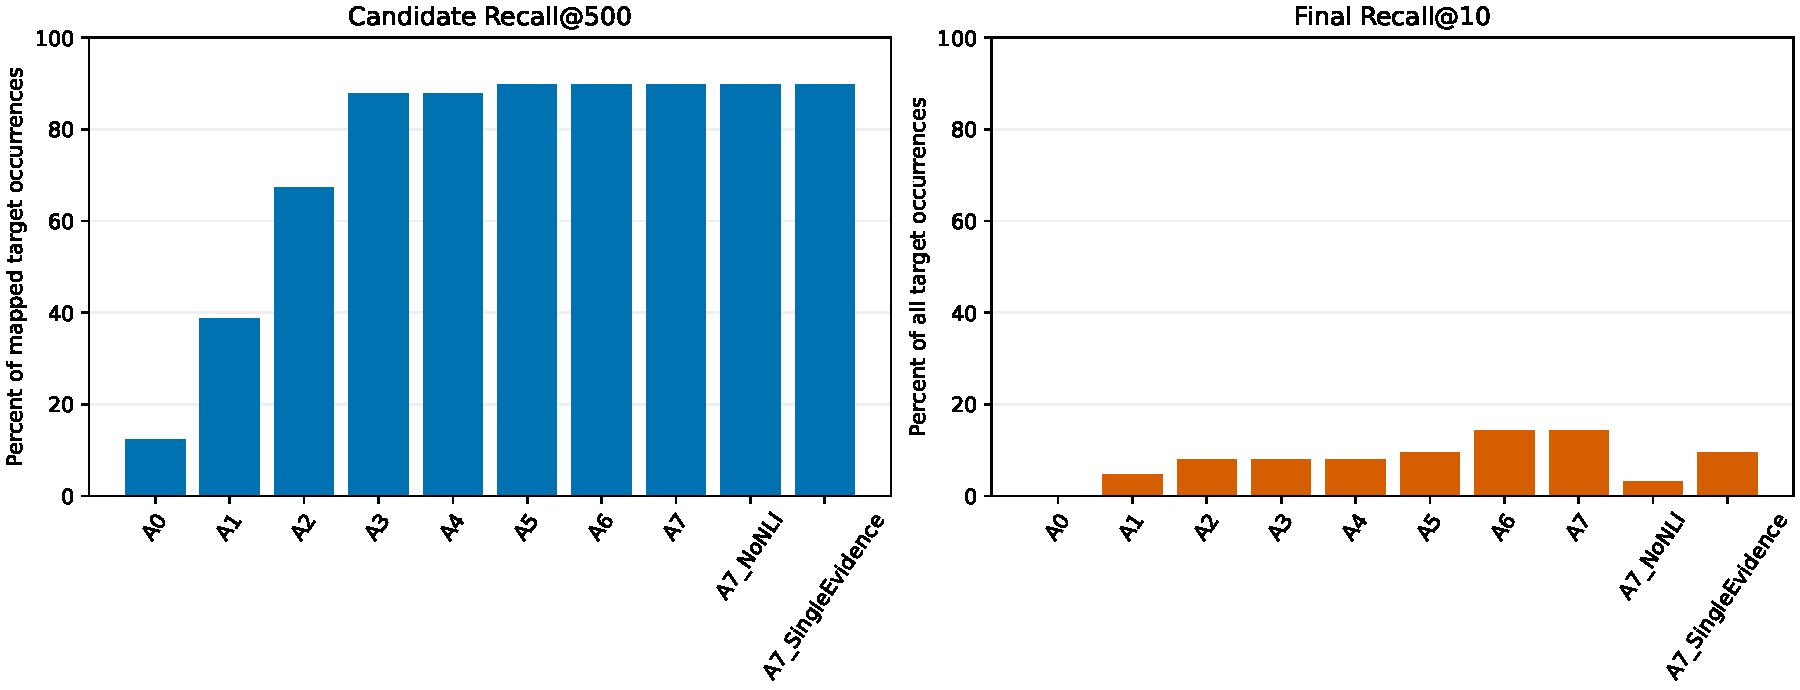
\includegraphics[width=0.92\textwidth]{stage_metrics.pdf}}{\framebox{\parbox{0.9\textwidth}{\centering\vspace{12mm}Figure file \path{stage_metrics.pdf} not present at compile time.\\ The figure compares candidate recall at 500 over 49 mapped targets with final recall at 10 over all 63 targets.\vspace{12mm}}}}
\caption{Candidate recall at 500 (left, denominator 49) and final recall at 10 (right, denominator 63). The panels have different denominators and measure different stages.}
\label{fig:stage}
\end{figure}

\paragraph{The primary system does not win, and that is reported as measured.} On this development benchmark A7 is not the best arm. Its MRR of 0.110 is below A6 (0.148), A5 (0.155), A4 (0.201), A3 (0.198), A2 (0.187), A1 and TypedRaw (0.167) and A6\_100 (0.167). Its recall at 100 of 29/63 is below A5 and A6\_100 (37/63) and A6 (33/63). Its conditional observed mean rank of 182.0 is worse than A5 and A6, and its penalised mean of 525.9 is correspondingly worse than A5's 430.9. A7 is marginally ahead of A6 at recall at 50 (23 versus 22 occurrences) and at the observed median (50.5 versus 51.5), and it matches A6 at 5, 10 and 25. Nothing was retuned in response to these numbers and no control is promoted to primary: A7 was declared primary in advance, so A7 remains the primary and the comparison stands as a negative result for the conjunction stage in its current form.

\paragraph{What the A7 controls do and do not show.} Both A7 controls are worse than A7: disabling the NLI tiers (A7\_NoNLI, MRR 0.065) and reducing evidence to $k=1$ (A7\_SingleEvidence, MRR 0.080). This says that within the A7 design the tier signal and the three-block evidence bundle both carry weight, and in particular that the measured A7 numbers are not an artefact of the tiers being inert. It does \emph{not} say that A7 is a good ranker, since the whole family remains behind the simpler A5 and A6 arms on MRR and recall at 100. The controls also differ in cost accounting: A7\_NoNLI reuses the already computed component relevance scores and is therefore not an independently timed model run, whereas A7\_SingleEvidence runs both models independently on $k=1$ bundles.

\paragraph{Depth of relevance re-scoring.} The relevance depth controls are informative in the opposite direction from the usual intuition: shallower re-scoring is better here. A6\_100 is the best relevance arm on MRR (0.167) and on hits at 10 (12 of 63), A6\_200 is intermediate, and A6 at depth 500 is the weakest of the three despite having the largest pool. Re-scoring a deeper prefix admits more opportunities for the relevance model to promote a plausible non-target above a target, which is visible directly in the movement tables below.

\subsection{Conditional movement under re-ranking}

\begin{table}[htbp]
\centering
\footnotesize
\caption{Movement of target occurrences seen inside each re-ranking pool, relative to the A5 fusion order. Medians are over the seen occurrences. Conditional recall at 10 is over the seen occurrences of that pool.}
\label{tab:movement}
\resizebox{\textwidth}{!}{%
\begin{tabular}{@{}lrrrrrrrrrr@{}}
\toprule
Arm & Pool & Seen & Up & Down & Unch. & Top10 after & New top10 & Left top10 & R@10 cond. & Median before $\to$ after \\
\midrule
A6\_100 & 100 & 37 & 17 & 20 & 0 & 12 & 7 & 1 & 0.324 & 36.0 $\to$ 27.0 \\
A6\_200 & 200 & 43 & 19 & 24 & 0 & 9 & 5 & 2 & 0.209 & 39.0 $\to$ 38.0 \\
A6 & 500 & 44 & 18 & 26 & 0 & 9 & 5 & 2 & 0.205 & 39.0 $\to$ 50.5 \\
A7 & 500 & 44 & 17 & 26 & 1 & 9 & 5 & 2 & 0.205 & 39.0 $\to$ 46.5 \\
A7\_NoNLI & 500 & 44 & 12 & 32 & 0 & 2 & 1 & 5 & 0.045 & 39.0 $\to$ 66.0 \\
A7\_SingleEvidence & 500 & 44 & 10 & 34 & 0 & 6 & 3 & 3 & 0.136 & 39.0 $\to$ 109.0 \\
\bottomrule
\end{tabular}}
\end{table}

Every re-ranking arm at depth 500 moves more target occurrences down than up. For A7, 17 occurrences improve, 26 worsen and 1 is unchanged, 5 occurrences enter the top 10 and 2 leave it, and the median seen rank degrades from 39.0 to 46.5 while the conditional recall at 10 is unchanged relative to A6. The counts of downward movement are counts of \emph{target} occurrences relative to the fusion order; they are not counts of entities that the requirement stage actively judged unsuitable, and the failure labels in Section~\ref{sec:failures} are likewise not demotion counts.

\begin{table}[htbp]
\centering
\footnotesize
\caption{A6 to A7 transition over the 44 seen target occurrences: the isolated effect of replacing global relevance ordering with the conjunction criterion on the same prefix.}
\label{tab:a6a7}
\begin{tabular}{@{}lrrrrrr@{}}
\toprule
Seen & Up & Down & Unchanged & New top10 & Left top10 & Median before $\to$ after \\
\midrule
44 & 18 & 25 & 1 & 4 & 4 & 50.5 $\to$ 46.5 \\
\bottomrule
\end{tabular}
\end{table}

The A6-to-A7 transition preserves recall at 10 but worsens MRR and recall at 100, with strongly varying effects per occurrence. Large gains and large losses coexist: on Q1, \emph{MACE} moves 174 $\to$ 43 and \emph{M3GNet} 51 $\to$ 34, while \emph{GAP} moves 3 $\to$ 42 and \emph{CHGNet} 31 $\to$ 107; on Q14, \emph{Materials Project} moves 49 $\to$ 2, \emph{WBM} 86 $\to$ 14 and \emph{OQMD} 67 $\to$ 19, while \emph{Matbench} moves 3 $\to$ 32 and \emph{MPtrj} 16 $\to$ 39; on Q12, \emph{UMA} moves 161 $\to$ 67 and \emph{DeePMD} 20 $\to$ 8, while \emph{NequIP} moves 65 $\to$ 486 and \emph{EquiformerV2} 37 $\to$ 419. Some large negative excursions coincide with proxy contradictions and tier 3, including Q12 NequIP. Other large losses, such as Q13 MACE, are labelled ranker failures without that flag. These traces suggest mechanisms but do not establish that the NLI judgments are scientifically wrong.

\subsection{Per-occurrence target ranks}

Table~\ref{tab:perq} lists every annotated Type-A target occurrence with its ranks in A5, A6, A7 and the two A7 controls, and its operational top-10 outcome label. Occurrences with a dash are not directly resolvable identities or were never retrieved. Two occurrences on Q13, \emph{MEGNet} at 733 and \emph{EquiformerV2} at 551, sit outside the 500-prefix and therefore keep an identical untouched fusion position in every re-ranking arm, which is the visible signature of the prefix/tail contract. Machine-readable traces for all occurrences and all components, including packed-bundle records and raw probabilities, accompany the frozen artefacts under \path{artifacts/prediction} and \path{artifacts/evaluation}.

\paragraph{Failure code mapping.} RF: requirement ranker failed; REM: requirement evidence missing; R10: recovered at 10; GTU: ground-truth mapping uncertain; CPX: contradiction proxy failure; ORP: outside rerank pool; WTY: wrong type filter. Exact machine-readable labels appear in Table~\ref{tab:failures}.

{\footnotesize
\begin{longtable}{@{}lp{3.0cm}lrrrrrl@{}}
\caption{All 63 annotated Type-A target occurrences with measured ranks. \texttt{NoNLI} and \texttt{SE} are A7\_NoNLI and A7\_SingleEvidence.}\label{tab:perq}\\
\toprule
Q & Target & Status & A5 & A6 & A7 & NoNLI & SE & Code \\
\midrule
\endfirsthead
\multicolumn{9}{l}{\footnotesize Table~\ref{tab:perq} continued.}\\
\toprule
Q & Target & Status & A5 & A6 & A7 & NoNLI & SE & Code \\
\midrule
\endhead
\midrule
\multicolumn{9}{r}{\footnotesize continued on next page}\\
\endfoot
\bottomrule
\endlastfoot
Q1 & MACE & EXACT & 39 & 174 & 43 & 69 & 67 & RF \\
Q1 & M3GNet & EXACT & 35 & 51 & 34 & 52 & 58 & RF \\
Q1 & CHGNet & EXACT & 72 & 31 & 107 & 122 & 115 & REM \\
Q1 & GAP & EXACT & 31 & 3 & 42 & 67 & 49 & RF \\
Q1 & NequIP & EXACT & 24 & 56 & 51 & 83 & 485 & RF \\
Q1 & ACE & EXACT & 159 & 370 & 415 & 447 & 491 & RF \\
Q1 & EquiformerV2 & EXACT & 23 & 54 & 30 & 45 & 42 & RF \\
Q2 & DeepH & EXACT & 40 & 15 & 7 & 65 & 10 & R10 \\
Q2 & D4FT & EXACT & 6 & 10 & 31 & 33 & 43 & RF \\
Q2 & HamGNN & PARTIAL & -- & -- & -- & -- & -- & GTU \\
Q3 & xDeepH & PARTIAL & -- & -- & -- & -- & -- & GTU \\
Q3 & DeepH-E3 & EXACT & 2 & 7 & 5 & 11 & 4 & R10 \\
Q4 & Hessian training & ALIAS & 44 & 229 & 195 & 237 & 198 & REM \\
Q4 & VGNN & EXACT & 33 & 69 & 441 & 61 & 445 & CPX \\
Q4 & MACE-F & ABSENT & -- & -- & -- & -- & -- & GTU \\
Q5 & Bead-mapping & ABSENT & -- & -- & -- & -- & -- & GTU \\
Q5 & GNN+GPP & PARTIAL & -- & -- & -- & -- & -- & GTU \\
Q6 & DeePMD+AL & PARTIAL & -- & -- & -- & -- & -- & GTU \\
Q6 & LiFlow & EXACT & 2 & 42 & 5 & 16 & 6 & R10 \\
Q6 & MLIP descriptors & PARTIAL & -- & -- & -- & -- & -- & GTU \\
Q7 & GNN free energies & PARTIAL & -- & -- & -- & -- & -- & GTU \\
Q7 & symbolic regression & EXACT & 48 & 276 & 495 & 484 & 498 & CPX \\
Q8 & ConvLSTM & EXACT & 7 & 6 & 4 & 18 & 3 & R10 \\
Q8 & GNN stress fields & PARTIAL & -- & -- & -- & -- & -- & GTU \\
Q9 & E(3)-equivariant GNNs & PARTIAL & -- & -- & -- & -- & -- & GTU \\
Q9 & physics-informed & PARTIAL & -- & -- & -- & -- & -- & GTU \\
Q9 & NequIP & EXACT & 256 & 60 & 54 & 464 & 476 & RF \\
Q10 & GNNs + ACE descriptors & PARTIAL & -- & -- & -- & -- & -- & GTU \\
Q10 & SchNet & EXACT & 156 & 87 & 441 & 437 & 468 & CPX \\
Q11 & CE$\to$MC$\to$NN$\to$PF & COMPOSITE & -- & -- & -- & -- & -- & GTU \\
Q11 & hybrid frameworks & PARTIAL & -- & -- & -- & -- & -- & GTU \\
Q12 & MACE & EXACT & 42 & 302 & 490 & 465 & 469 & CPX \\
Q12 & NequIP & EXACT & 39 & 65 & 486 & 447 & 485 & CPX \\
Q12 & CHGNet & EXACT & 94 & 38 & 92 & 100 & 95 & REM \\
Q12 & M3GNet & EXACT & 36 & 108 & 420 & 431 & 439 & RF \\
Q12 & SevenNet & EXACT & 40 & 50 & 50 & 52 & 13 & RF \\
Q12 & GAP & EXACT & 50 & 5 & 7 & 12 & 8 & R10 \\
Q12 & DeePMD & EXACT & 62 & 20 & 8 & 13 & 7 & R10 \\
Q12 & MatterSim & EXACT & 2 & 24 & 12 & 54 & 11 & RF \\
Q12 & Orb & EXACT & 26 & 52 & 100 & 108 & 103 & REM \\
Q12 & eSEN & EXACT & 12 & 99 & 424 & 436 & 426 & RF \\
Q12 & PET & EXACT & 61 & 317 & 498 & 495 & 474 & CPX \\
Q12 & UMA & EXACT & 67 & 161 & 67 & 74 & 489 & RF \\
Q12 & EquiformerV2 & EXACT & 57 & 37 & 419 & 430 & 14 & RF \\
Q13 & CGCNN & EXACT & 118 & 17 & 22 & 23 & 22 & RF \\
Q13 & SchNet & EXACT & 115 & 198 & 447 & 454 & 438 & RF \\
Q13 & MEGNet & EXACT & 733 & 733 & 733 & 733 & 733 & ORP \\
Q13 & M3GNet & EXACT & 95 & 142 & 39 & 41 & 41 & RF \\
Q13 & NequIP & EXACT & 89 & 121 & 435 & 440 & 467 & RF \\
Q13 & MACE & EXACT & 136 & 50 & 462 & 471 & 469 & RF \\
Q13 & CHGNet & EXACT & 113 & 35 & 80 & 85 & 78 & REM \\
Q13 & EquiformerV2 & EXACT & 551 & 551 & 551 & 551 & 551 & ORP \\
Q14 & Matbench Discovery & EXACT & 4 & 1 & 3 & 2 & 21 & R10 \\
Q14 & Matbench & EXACT & 39 & 3 & 32 & 33 & 33 & REM \\
Q14 & JARVIS-DFT & EXACT & -- & -- & -- & -- & -- & WTY \\
Q14 & Materials Project & EXACT & 15 & 49 & 2 & 13 & 327 & R10 \\
Q14 & MPtrj & EXACT & 37 & 16 & 39 & 40 & 40 & REM \\
Q14 & OQMD & EXACT & 33 & 67 & 19 & 20 & 322 & RF \\
Q14 & AFLOW & EXACT & -- & -- & -- & -- & -- & WTY \\
Q14 & Alexandria & EXACT & -- & -- & -- & -- & -- & WTY \\
Q14 & GNoME & EXACT & 26 & 10 & 6 & 5 & 349 & R10 \\
Q14 & WBM & EXACT & 29 & 86 & 14 & 15 & 326 & RF \\
Q14 & OMat24 & EXACT & 21 & 4 & 17 & 18 & 330 & RF \\
\end{longtable}}

\subsection{Requirement diagnostics}

\begin{table}[htbp]
\centering
\footnotesize
\caption{Requirement-stage diagnostics over all 18 questions. Candidates are candidate-question pairs inside the primary prefix; components are candidate-question-component triples. These are work counts, not target occurrences.}
\label{tab:reqdiag}
\begin{tabular}{@{}lr@{}}
\toprule
Quantity & Count \\
\midrule
Candidate-question pairs scored & 8849 \\
Component instances evaluated & 20349 \\
\midrule
Components \texttt{SUPPORTED} & 664 \\
Components \texttt{NOT\_SUPPORTED\_BY\_}\allowbreak\texttt{AVAILABLE\_EVIDENCE} & 18369 \\
Components \texttt{CONTRADICTED} & 1316 \\
\midrule
Tier 0 (all positive components supported, no contradiction) & 61 \\
Tier 1 (some positive support, no contradiction) & 268 \\
Tier 2 (no contradiction, no confident support) & 7564 \\
Tier 3 (any contradiction) & 956 \\
\midrule
Components with no evidence at all & 13558 \\
Components with no packed NLI evidence & 13558 \\
Components with imputed neutral-midpoint relevance rank & 13558 \\
Components with multiple \emph{selected} evidence blocks & 4839 \\
Components with multiple \emph{actually packed} NLI evidence blocks & 4839 \\
Components whose status differs between $k=3$ and $k=1$ & 1117 \\
\bottomrule
\end{tabular}
\end{table}

Three features of Table~\ref{tab:reqdiag} govern the interpretation of every A7 number.

First, \textbf{the evidence floor dominates}. 13558 of 20349 component instances, about two thirds, have no evidence, so their relevance rank is the fixed neutral midpoint and their status is \texttt{NOT\_SUPPORTED\_BY\_}\allowbreak\texttt{AVAILABLE\_EVIDENCE}. For those components the criterion is not measuring support at all; it is applying a convention. Missing is not false, but it is also not informative, and with this much missingness the ordering inside tier 2 is substantially driven by the imputation.

Second, \textbf{selected and packed multi-evidence counts coincide exactly} at 4839, and the no-packed count coincides with the missing count at 13558. Every nonempty selection retained some NLI evidence, and every multi-item selection retained multiple items. These counts do not prove that every selected item survived packing; the per-bundle packing records remain the authority.

Third, \textbf{tiering is sparse and contradiction is comparatively common}. Only 61 candidate-question pairs achieve tier 0 and 268 tier 1, against 956 in tier 3. Since tier 3 is strictly worse than tier 2 in the lexicographic order, a single uncalibrated contradiction sends a candidate behind every uninformative candidate. That is the intended semantics of a conjunction, and it is also the most plausible mechanism behind the large negative excursions in Table~\ref{tab:a6a7} and behind the 6 occurrences labelled \texttt{CONTRADICTION\_PROXY\_FAILURE}.

\paragraph{Top-3 versus top-1 evidence: status is unstable.} 1117 component instances change status when the bundle changes from three evidence blocks to one. Four frozen examples from Q1 show the mechanism and its direction is not uniform:

\begin{itemize}
\item \emph{Machine-learned interatomic potentials} against the component \emph{accuracy close to DFT}: with three blocks the proxy returns neutral 0.875, entailment 0.122, hence \texttt{NOT\_SUPPORTED\_BY\_}\allowbreak\texttt{AVAILABLE\_EVIDENCE}; with one block it returns entailment 0.991, hence \texttt{SUPPORTED}. The single block is the one claim that mentions DFT force accuracy directly; the longer premise changes the model output substantially; this does not establish a causal account of its internal reasoning.
\item \emph{Gaussian Approximation Potential (GAP) for silicon} against \emph{accuracy close to DFT}: three blocks give entailment 0.030 and neutral 0.969 (unsupported) while one block gives entailment 0.995 (supported), even though all three selected blocks are GAP-specific DFT-accuracy claims.
\item \emph{Gaussian Approximation Potential (GAP) for silicon} against \emph{computational efficiency}: the direction reverses. Three blocks give entailment 0.987 (\texttt{SUPPORTED}); one block gives contradiction 0.309, entailment 0.143, neutral 0.548 (unsupported).
\item \emph{Matbench Discovery} against \emph{computational efficiency}: three blocks give neutral 0.738 (unsupported), one block gives entailment 0.928 (supported), on evidence about rolling MAE computation and benchmarking that does not in fact assert efficiency of the benchmark itself.
\end{itemize}

These are not validated scientific judgements in either direction. They show that a small pretrained NLI model is sensitive to premise composition, and they are the reason the report treats every status as a proxy rather than a measurement of suitability. They also illustrate the parser limitation: \emph{computational efficiency} as a literal span loses the pre-head specificity of the original clause, and a candidate can appear to satisfy it on generic evidence.

\subsection{Failure categories}
\label{sec:failures}

Labels are assigned by a fixed precedence: temporal, uncertain mapping, no index, type filter, recovered at 10, not in union, outside pool, contradiction proxy flag, missing requirement evidence, remaining requirement ranker failure. \textbf{These are operational outcome labels for the primary arm, not established causes and not human scientific adjudications.} In particular, a \texttt{CONTRADICTION\_PROXY\_FAILURE} label means that an annotated missed target received a proxy contradiction; it is not proof that the NLI judgement is wrong. A counterfactual rank gain or loss does not adjudicate whether the non-gold entities ranked above a target are valid scientific alternatives, and the aggregate label counts are not counts of entities demoted by the requirement stage.

\begin{table}[htbp]
\centering
\footnotesize
\caption{Primary failure labels over all 63 Type-A target occurrences, and secondary flags. The seven primary categories partition the 63 occurrences.}
\label{tab:failures}
\begin{tabular}{@{}llr@{}}
\toprule
Code & Label & Occurrences \\
\midrule
RF & \texttt{REQUIREMENT\_RANKER\_FAILED} & 22 \\
GTU & \texttt{GROUND\_TRUTH\_MAPPING\_UNCERTAIN} & 14 \\
R10 & \texttt{RECOVERED\_AT\_10} & 9 \\
REM & \texttt{REQUIREMENT\_EVIDENCE\_MISSING} & 7 \\
CPX & \texttt{CONTRADICTION\_PROXY\_FAILURE} & 6 \\
WTY & \texttt{WRONG\_TYPE\_FILTER} & 3 \\
ORP & \texttt{OUTSIDE\_RERANK\_POOL} & 2 \\
\midrule
\multicolumn{2}{@{}l}{Secondary: \texttt{NO\_NAME\_MATCH}} & 46 \\
\multicolumn{2}{@{}l}{Secondary: \texttt{NO\_RELEVANT\_EVIDENCE}} & 8 \\
\bottomrule
\end{tabular}
\end{table}

The distribution is consistent with the rest of the measurements. 14 of 63 occurrences are not directly resolvable identities at all, which caps direct recall at 49/63 by construction before any retrieval happens. 9 occurrences are recovered in the primary top 10, matching the 9 direct hits at 10 in A7. 3 occurrences (\emph{JARVIS-DFT}, \emph{AFLOW}, \emph{Alexandria}, all on the dataset/benchmark question) are excluded by the answer-family filter, a declared precision constraint paying a recall cost because the indexed types do not match the requested family. 2 occurrences sit outside the 500-prefix and are untouched. The remaining 35 are distributed over ranker failure, missing requirement evidence and contradiction flags, and the secondary \texttt{NO\_NAME\_MATCH} flag appears on 46 occurrences; the name channel independently recovers zero mapped target occurrences in this benchmark.

\subsection{Efficiency}
\label{sec:efficiency}

\begin{table}[htbp]
\centering
\footnotesize
\caption{Logical work and actual inference. Logical counts describe all pairs implied by the design; actual counts are cache misses only. Wall times are descriptive single-machine measurements, not production latency.}
\label{tab:efficiency}
\begin{tabular}{@{}lr@{}}
\toprule
Quantity & Value \\
\midrule
Dense comparisons & 295920 \\
Evidence comparisons & 153864 \\
BM25 document-term lookups (exact) & 1637900 \\
Global relevance pairs (logical) & 8849 \\
Global relevance pairs actually inferred & 1500 \\
Global relevance wall time (s) & 102.2 \\
\midrule
A7: requirement dense comparisons & 175234 \\
A7: component relevance pairs (logical) & 6791 \\
A7: component relevance pairs actually inferred & 1422 \\
A7: NLI pairs (logical) & 6791 \\
A7: NLI pairs actually inferred & 1422 \\
A7: arm wall time (s) & 232.7 \\
\midrule
A7\_SingleEvidence: requirement dense comparisons & 175234 \\
A7\_SingleEvidence: relevance and NLI pairs (logical, each) & 6791 \\
A7\_SingleEvidence: relevance and NLI pairs actually inferred (each) & 1422 \\
A7\_SingleEvidence: arm wall time (s) & 119.6 \\
\midrule
Evaluated-stage wall time (s) & 471.1 \\
Prediction process wall time (s), exit code 0 & 601.6 \\
\bottomrule
\end{tabular}
\end{table}

The gap between logical and actual counts is the honest headline of this table: 1500 of 8849 global relevance pairs and 1422 of 6791 requirement pairs per arm were actually inferred, because this run reuses cached pure-model scores computed before the tier clarification. The timings are therefore mixed cold/cached and \emph{understate} a from-scratch run; they must not be read as uncached inference cost or as production latency. A7\_SingleEvidence shows a lower wall time than A7 at identical logical and actual pair counts, which is consistent with shorter packed premises, but this single mixed-cache run does not isolate the cause of the timing difference. A7\_NoNLI is not listed because it shares the already computed component relevance scores and runs no NLI, so it has no independently timed model cost; similarly, the A6\_100 and A6\_200 controls reuse the 500-pool global relevance scores. Interrupted pre-evaluation invocations produced no freeze and no gold evaluation and are excluded from these totals; they also performed no empirical selection.

\section{Discussion}

The measurements support a narrow, concrete reading and nothing wider.

\textbf{Recall is a channel problem and it responded to channel breadth.} Moving from a V1-like raw dense arm to a typed multi-channel union with evidence owners and a bounded graph channel raised mapped pool recovery from 6/49 to 46/49, and fusion concentrated that recovery at shallow cutoffs. This is the clearest positive result in the run. It is still a retrieval result on a small development benchmark and says nothing about abstraction quality.

\textbf{The conjunction stage is dispersive, and in aggregate it costs more than it gains here.} A7 improves 17 of 44 seen occurrences and worsens 26, and ends behind A5 and A6 on MRR and recall at 100. Its two controls are worse than it is, so the tiers and the three-block bundles are doing work; the work is simply not net positive at this evidence density. Two measured conditions plausibly bound it: two thirds of component instances have no evidence and are decided by a fixed imputation, and a single uncalibrated contradiction is lexicographically fatal. Both are design choices stated in advance, and both are candidates for the first follow-up experiments rather than for post-hoc retuning.

\textbf{Depth hurts relevance re-ranking here.} A6\_100 outperforms A6\_200 and A6 at depth 500. A deeper prefix gives both re-rankers more opportunities to promote plausible non-targets.

\textbf{What is not claimed.} V2 does not solve conditional entity retrieval; the highest recall at 100 is 37/63 (A5 and A6\_100), while the highest MRR is about 0.20 (A4). These maxima belong to different arms. Higher flat recall is not evidence of better abstraction or of hierarchy acceleration. Requirement support is not expert validation. Publication-year visibility is not temporal stability. A status change is not a validated improvement, and a cached replay is not an independent run.

\section{Limitations}

\begin{itemize}
\item \textbf{Benchmark size and exposure.} 18 questions, 14 Type-A, 63 target occurrences; no new expert re-annotation was performed. All results are development results; the freeze blocks run-time gold access, not design-time exposure.
\item \textbf{Mapping ceilings.} 14 of 63 occurrences are \texttt{PARTIAL}, \texttt{ABSENT} or \texttt{COMPOSITE} and can never receive direct credit, capping direct recall at 49/63.
\item \textbf{Evidence sparsity.} 2508 of 2978 entities have no candidate-specific evidence; 13558 of 20349 component instances are decided by the fixed neutral-midpoint imputation.
\item \textbf{Fixed aggregation and imputation.} The lexicographic order, the geometric mean, the weakest-component term and the midpoint convention are declared a priori and unoptimised. They are assumptions, not results, and the midpoint convention lets evidence-free candidates outrank weakly evidenced ones.
\item \textbf{Proxy calibration.} Both cross-encoders emit uncalibrated scores. The 0.7/0.3 thresholds are frozen defaults, not calibrated operating points, and tier 3 is strictly dominant in the order.
\item \textbf{Heuristic parser.} Literal span extraction can split compounds imperfectly, can extract problem phrases ambiguously and leaves pre-head modifiers unseparated, so component sets can be less specific than the question.
\item \textbf{Year precision and inferred roles.} Visibility is year-level, so month constraints are unresolvable; relation roles come from the supplied graph.
\item \textbf{Pretrained domain mismatch.} All three models are general-purpose and none was adapted to materials science text.
\item \textbf{Single hardware, single seed.} One 4-thread CPU configuration, seed 42, no seed sweep and no confidence intervals on any arm difference. The arm differences in Table~\ref{tab:final} are measured point values on 14 questions and are not accompanied by uncertainty estimates.
\item \textbf{Timing caveats.} Mixed cold/cached inference; NLI determinism is untested; the competition-rank routine is $O(mK^2)$ in pure Python.
\item \textbf{Scope.} No hierarchy is built, traversed or evaluated; no P1--P6 or T1--T5 compliance is claimed.
\end{itemize}

\section{Reproducibility}

The V2 repository contains the exact commands, pinned dependencies, pinned model revisions, the fixed \path{config.json} reproduced in part in Table~\ref{tab:models}, the test suite and the recorded hashes. The two-process contract is: run \path{predict.py} to produce and freeze \path{artifacts/prediction}; run \path{evaluate.py}, which verifies every hash before importing or reading gold and re-verifies afterwards, to produce \path{artifacts/evaluation}. The frozen prediction digest is quoted in Section~\ref{sec:freeze}. The access audit for the frozen run records 0 denied reads, 0 gold reads and 0 historical evaluation reads over 4186 project reads, with 15 local V2 modules imported.

Only V2 was modified in this task. The superseded top-20 verification code and the unused legacy candidate and evaluator modules were removed rather than kept for backward compatibility. The active phase outputs are \path{artifacts/prediction} and \path{artifacts/evaluation} inside the same existing V2 project, not a new experiment tree; an attempted bulk deletion of older V2 directories was automatically blocked, so those older artefacts remain present but inactive and access-denied to the predictor. V1 began this task with two tracked report changes and four untracked files, which the user approved preserving; protected-hash comparisons are made against that start state rather than against \texttt{HEAD}, and \path{rest_of_work} is hashed in full (86667 files). \textbf{Zero new changes were made to V1 or to \path{rest_of_work}}, and no GitHub operation of any kind was performed.

\section{AI usage disclosure}

This work was produced with AI assistance, declared in full and recorded with per-call detail in the V2 \path{AI_USAGE.md}, which lists prompts, accepted and rejected advice and the verification performed.

\begin{itemize}
\item \textbf{Codex} implemented, integrated and executed the pipeline, ran the frozen prediction and evaluation, measured every number reported here, validated the artefacts, and supplies the factual corrections, layout fixes and LaTeX compilation of this document.
\item \textbf{Claude Opus 5} was used for planning and compliance consultation, including the review of the original assessment brief that produced the scope matrix.
\item \textbf{Claude Sonnet 5} was used for optional code review.
\item \textbf{Claude Opus 5} authored this report and the companion from the frozen handoff, without executing code or reading results beyond the handoff.
\end{itemize}

The positive-only reading of tier 1 was a semantics correction adopted before the freeze and before evaluation, on reviewer advice and never from gold labels. No primary predictive policy was changed after the current evaluation results were read. \textbf{There was no human expert adjudication of any result in this report}, and helper models, their advice and their errors are recorded honestly in the JSON logs rather than paraphrased favourably.

\section{Four more weeks}

In priority order, and with no expectation that any of them would favour the current primary arm:

\begin{enumerate}
\item \textbf{Calibrate or replace the support proxy.} Sample component instances across all four tiers, obtain human adjudication, and measure the proxy's precision for \texttt{CONTRADICTED} in particular, since tier 3 is lexicographically fatal. Consider softening tier 3 to a bounded penalty only if calibration justifies it, declared in advance.
\item \textbf{Attack the evidence floor.} 13558 imputed component instances dominate the criterion. Measure sensitivity of every A7 number to the imputation convention (midpoint, worst, drop-component) as a declared sensitivity study rather than a selection.
\item \textbf{Declare and run a matched hierarchy-versus-flat comparison} with identical eligible entities, evidence, scorers, snapshot, mapping and cost accounting, fixed before scoring, to address the extrinsic question honestly.
\item \textbf{Enlarge and re-annotate the benchmark}, with multiple annotators, explicit adjudication of \texttt{PARTIAL} and \texttt{COMPOSITE} targets, and a genuinely held-out split.
\item \textbf{Seed and perturbation sweeps with intervals} so that differences such as A7 versus A6 can be reported with uncertainty rather than as point values.
\item \textbf{Engineering and verification.} An uncached timing run, an $O(mK\log K)$ rank routine, explicit NLI determinism tests, and a review of the answer-family filter that currently excludes three dataset targets.
\end{enumerate}

\section{Verification summary}

Codex verified the final test, access, replay and protected-tree records after the report draft. The measured tallies follow.

\IfFileExists{verification_summary.tex}{The complete V2 suite passed: \textbf{57 tests passed, zero failed and zero skipped}, in 812.27 seconds. Most elapsed time was the full protected-directory content audit. Tests cover entity/time/type/name/BM25/graph/RRF invariants, original text and source spans, owned evidence selection and packing, requirement aggregation and exclusions, missing-data semantics, prediction access isolation, freeze-before-gold, frozen-file protection and deterministic cached replay.

All 1,056 files under \texttt{clean\_tshc} and 86,667 files under \texttt{rest\_of\_work} match their initial SHA-256 hashes; protected git diffs and status entries also match. There are \textbf{zero new protected-tree changes}. The user's pre-existing V1 work is preserved.

The prediction access audit records zero gold or historical-result reads and no denied reads. Evaluation-only positive controls pass. Primary and cached replay prediction SHA-256 values match, and the registered predictive policy remains unchanged after evaluation. A cached replay does not establish independent uncached NLI determinism. No model was trained, fitted or tuned against benchmark gold, and no GitHub action was taken.

The exact file inventory, test log, protected-tree comparison, report checks and final artifact hashes are under \path{artifacts/verification/}. These checks establish local consistency and preserve the development-only interpretation.
}{}

\end{document}
